\documentclass{beamer}

\usetheme{CambridgeUS}
\usecolortheme{orchid}

\usepackage{inconsolata}

\usepackage{tikz}
\usetikzlibrary{shapes.geometric, positioning}

\begin{document}

\title[Spline mesh for wind turbine blades]{Spline based mesh generator for wind turbine blades}
\author[E. Fonn]{
  E.~Fonn\inst{1,2} \and
  A.~Rasheed\inst{2} \and
  A.~M.~Kvarving\inst{2} \and
  T.~Kvamsdal\inst{2,3}
}
\institute[SINTEF]{
  \inst{1}%
  \url{eivind.fonn@sintef.no}
  \and
  \inst{2}%
  Applied Mathematics, SINTEF ICT \\ \url{http://www.sintef.no}
  \and
  \inst{3}%
  Department of Mathematical Sciences, NTNU
}
\date[27th NCSM, 2014]{}

\titlegraphic{
  \includegraphics[width=0.3\textwidth]{common/sintef}
  \hspace{0.3cm}
  \includegraphics[width=0.22\textwidth]{common/ntnu}
}

\begin{frame}
  \titlepage
\end{frame}

\section{The NREL 5MW blade}

\begin{frame}
  \frametitle{The NREL 5MW reference blade}

  Cross sections defined at certain points along the radial axis (wingfoil shape, aerodynamic
  origin, twist angle, chord length, etc.)

  \begin{figure}
    \centering
    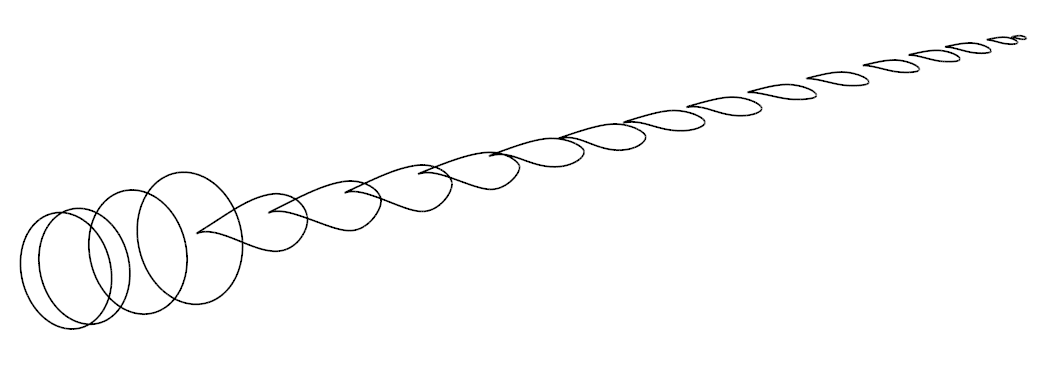
\includegraphics[width=0.8\textwidth]{figs/cross-airfoils}
  \end{figure}
\end{frame}

\begin{frame}
  \frametitle{Trailing edges}

  The airfoils are non-periodic spline curves with sharp trailing edges.

  \begin{figure}
    \centering
    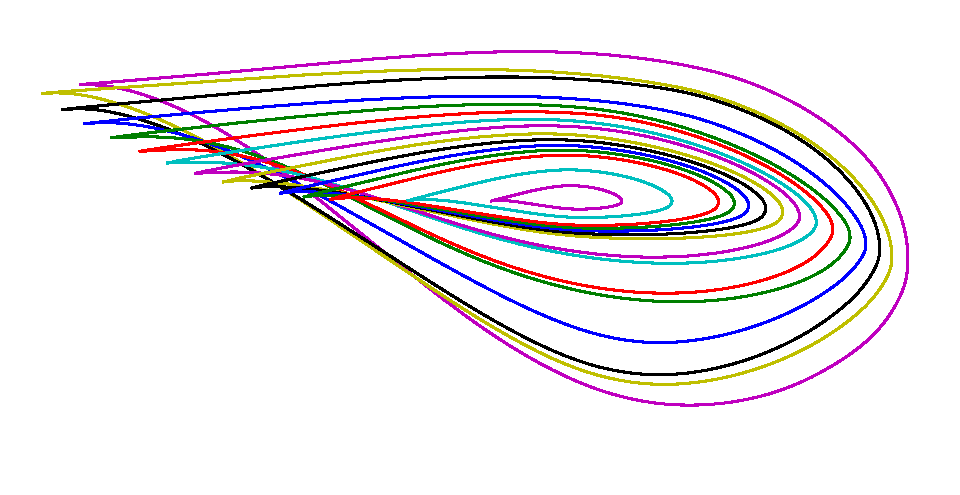
\includegraphics[width=0.8\textwidth]{figs/airfoils-note}
  \end{figure}
\end{frame}

\begin{frame}
  \frametitle{C-meshes}

  Typically, this forces a ``C''-mesh type construction.

  \begin{figure}
    \centering
    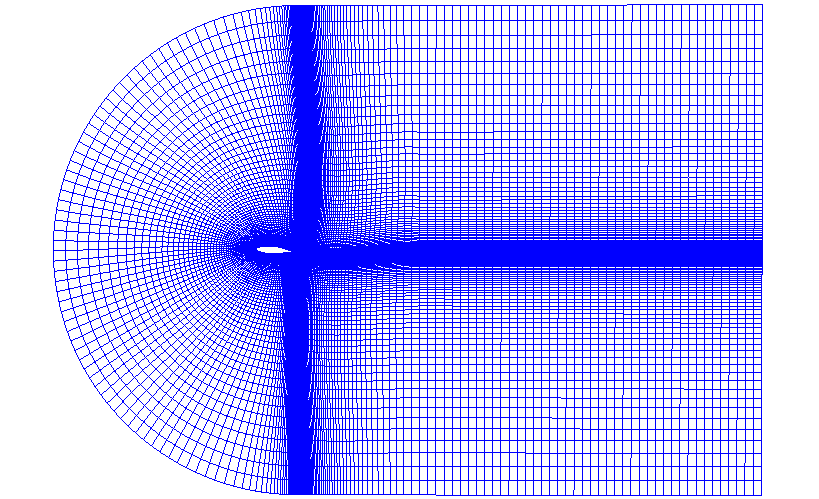
\includegraphics[width=0.7\textwidth]{figs/Sec41_a8_mesh}
  \end{figure}
\end{frame}

\begin{frame}
  \frametitle{Rounded trailing edge modification}

  Instead, we modify the foils slightly to allow for a rounded trailing edge.

  \begin{figure}
    \centering
    \only<1>{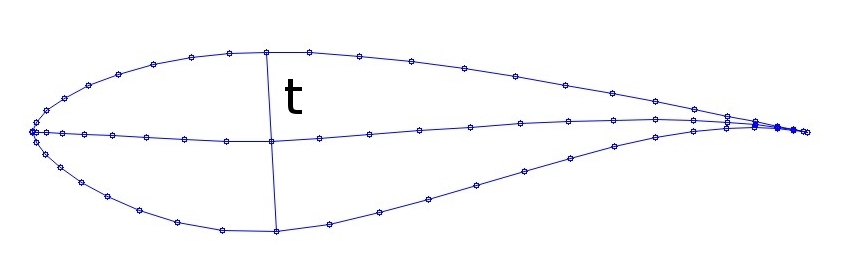
\includegraphics[width=0.7\textwidth]{figs/wingpoints_midline_normal}}
    \only<2>{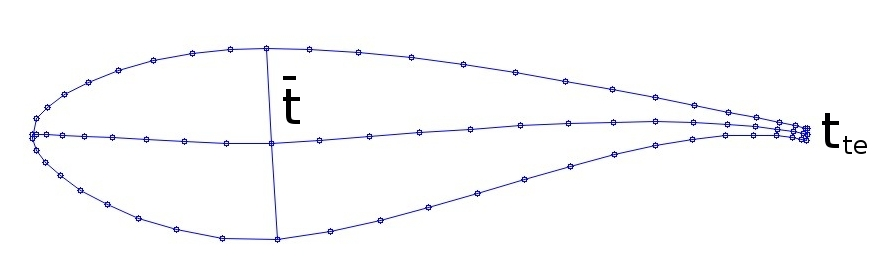
\includegraphics[width=0.7\textwidth]{figs/wingpoints_gap}}
    \only<3>{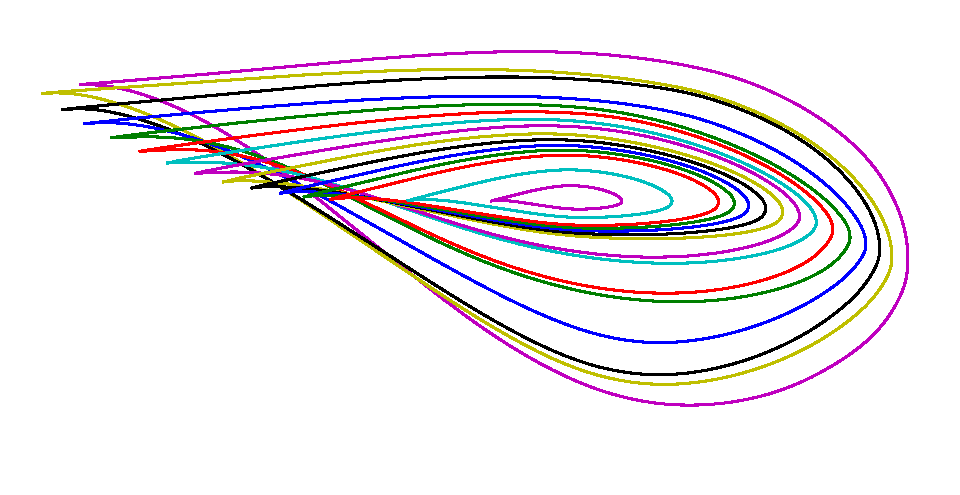
\includegraphics[width=0.7\textwidth]{figs/airfoils-te}}
    \only<1>{\caption{Before.}}
    \only<2-3>{\caption{After (exaggerated.)}}
  \end{figure}
\end{frame}

\begin{frame}
  \frametitle{O-meshes}

  This should allow us to create an ``O''-mesh instead, which is more efficient.

  \begin{figure}
    \centering
    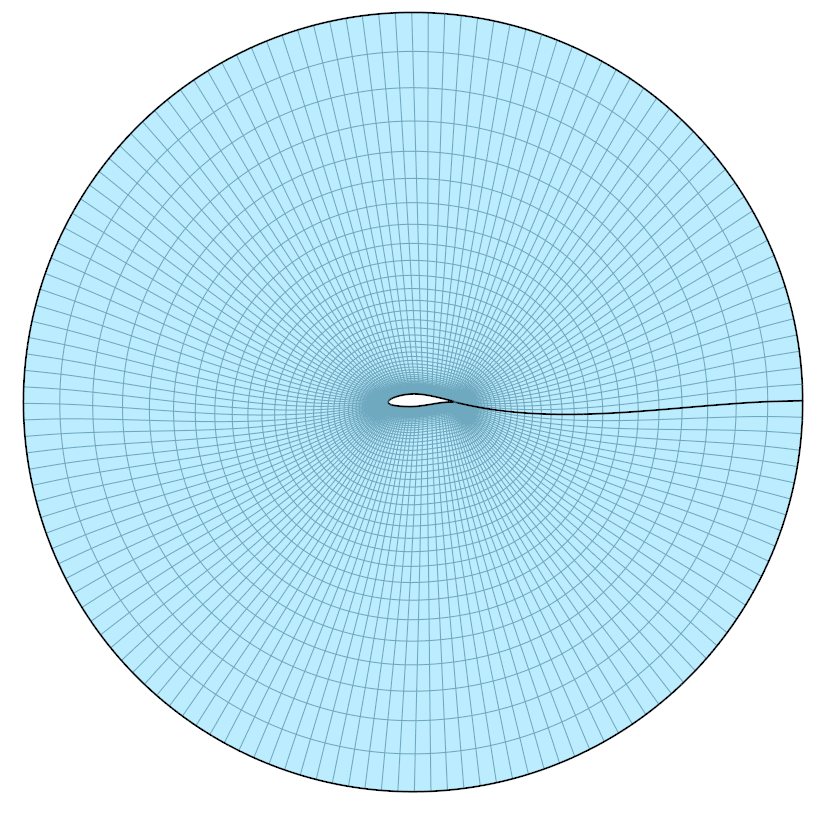
\includegraphics[width=0.4\textwidth]{figs/omesh}
  \end{figure}
\end{frame}

\section{Transfinite interpolation}
\subsection{Linear}

\begin{frame}
  \frametitle{Transfinite interpolation}

  Useful tool for ``filling in'' geometry.  Works for any parametrizations, not just splines.
  
  \begin{itemize}
  \item Four curves $\rightarrow$ surface.
  \item Six surfaces $\rightarrow$ volume.
  \item Twelve curves $\rightarrow$ volume.
  \item Etc.
  \end{itemize}
\end{frame}

\begin{frame}
  \frametitle{Four edges $\rightarrow$ surface}

  Given curves $\mathbf{c}_1, \ldots, \mathbf{c}_4$ with parameter domains $[0,1]$.

  \begin{figure}
    \centering
    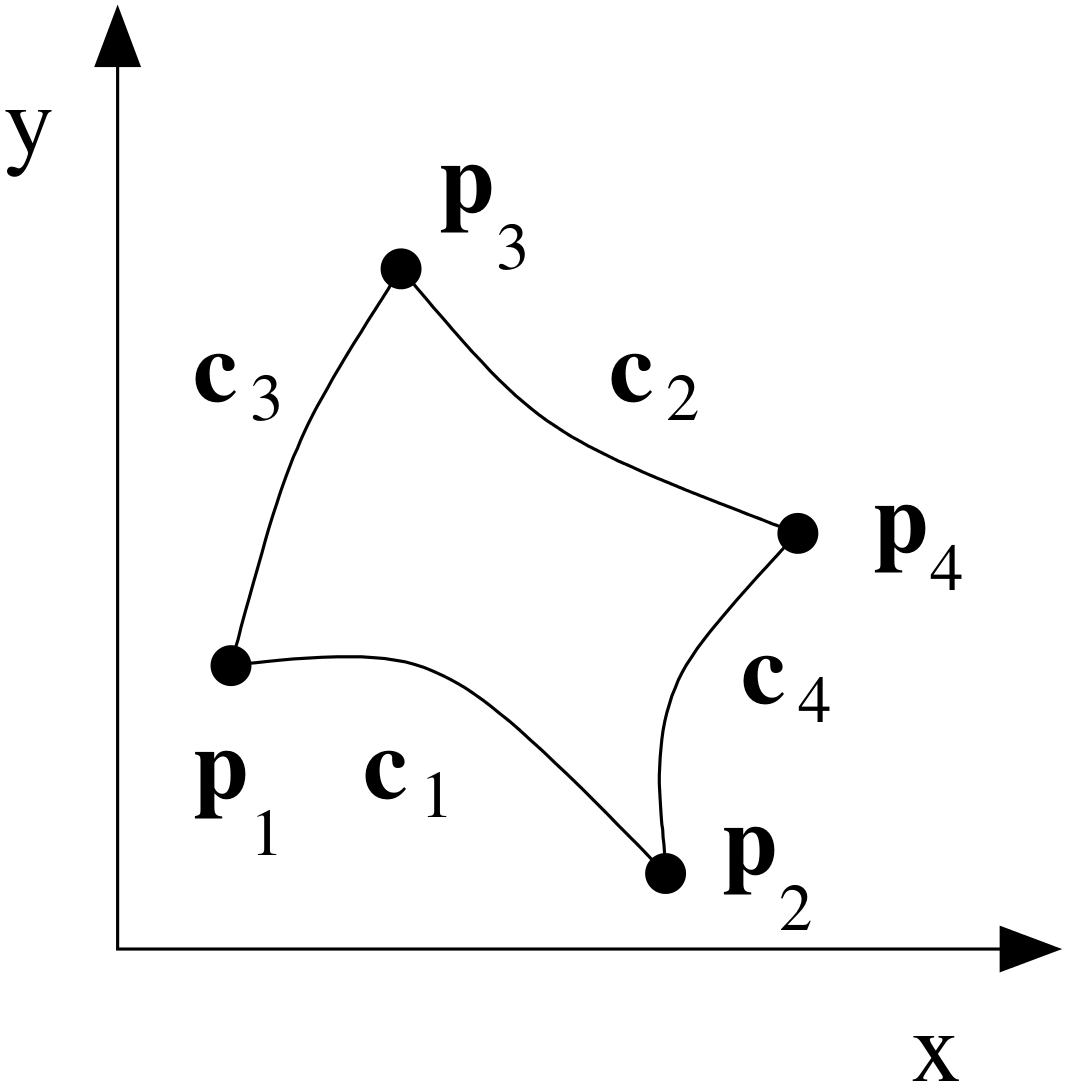
\includegraphics[width=0.4\textwidth]{figs/tfi}
  \end{figure}
\end{frame}

\begin{frame}
  \frametitle{Four edges $\rightarrow$ surface}

  The value of the surface at any point $(u,v) \in [0,1]^2$ is then

  \begin{align*}
    S(u,v) &= (1-v)\mathbf{c}_1(u) + v\mathbf{c}_2(u) \\
    &+ (1-u)\mathbf{c}_3(v) + u\mathbf{c}_4(v) \\
    &- (1-u)(1-v)\mathbf{p}_1 - uv\mathbf{p}_4 \\
    &- (1-u)v\mathbf{p}_3 - u(1-v)\mathbf{p}_2.
  \end{align*}

  Note: for $u\in\{0,1\}$ or $v\in\{0,1\}$, the parametrization of the edges behaves as expected.
\end{frame}

\begin{frame}
  \frametitle{Four edges $\rightarrow$ surface}

  \begin{figure}
    \centering
    \only<1>{
      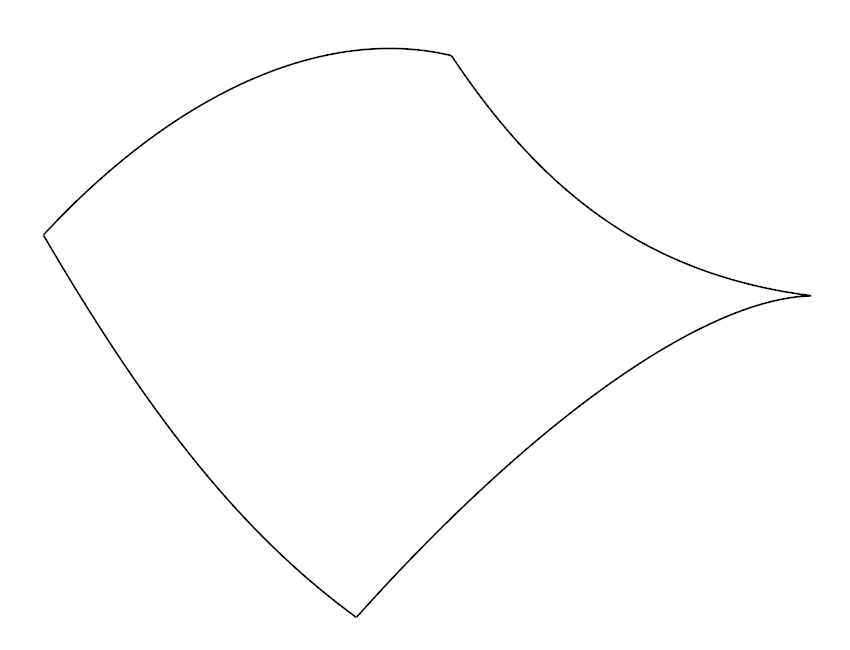
\includegraphics[width=0.6\textwidth]{figs/tfi-before}
      \caption{Before}
    }
    \only<2>{
      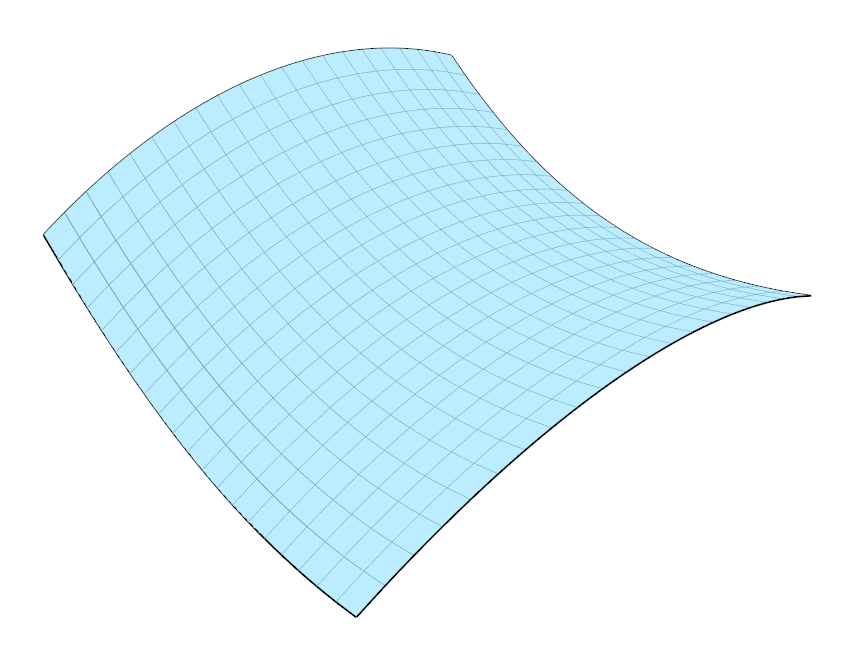
\includegraphics[width=0.6\textwidth]{figs/tfi-after}
      \caption{After}
    }
  \end{figure}
\end{frame}

\begin{frame}
  \frametitle{Parameter-normalized TFI}

  Problem: The parametrization of the edge curves will have a large impact on the distribution of
  nodes within the surface.  This can give awkward-looking results. \\~\\

  To prevent this, we want to normalize according to curvelength.  However, it's not guaranteed that
  the nodes of opposite curves are located at the same (normalized) curvelength parameters.
\end{frame}

\begin{frame}
  \frametitle{Parameter-normalized TFI}

  \begin{figure}
    \centering
    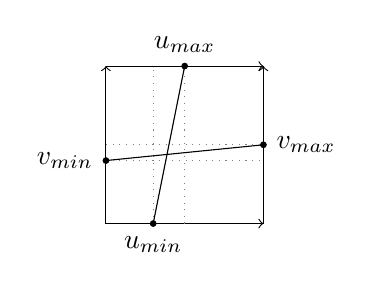
\begin{tikzpicture}[scale=2]
      \draw[->] (0,0) -- (1,0);
      \draw[->] (0,1) -- (1,1);

      \draw[->] (0,0) -- (0,1);
      \draw[->] (1,0) -- (1,1);
      \draw (0.3,0) -- (0.5,1);
      \draw[dotted, gray] (0.3,0) -- (0.3,1);
      \draw[dotted, gray] (0.5,0) -- (0.5,1);
      \draw (0,0.4) -- (1,0.5);
      \draw[dotted, gray] (0,0.4) -- (1,0.4);
      \draw[dotted, gray] (0,0.5) -- (1,0.5);
      \node [label=below:$u_\text{min}$, draw, fill=black, circle, inner sep=0pt, minimum size=2] at (0.3,0) {};
      \node [label=above:$u_\text{max}$, draw, fill=black, circle, inner sep=0pt, minimum size=2] at (0.5,1) {};
      \node [label=left:$v_\text{min}$, draw, fill=black, circle, inner sep=0pt, minimum size=2] at (0,0.4) {};
      \node [label=right:$v_\text{max}$, draw, fill=black, circle, inner sep=0pt, minimum size=2] at (1,0.5) {};
    \end{tikzpicture}
  \end{figure}

  \only<1>{
    \begin{align*}
      u &= u_\text{min} + v\underbrace{(u_\text{max} - u_\text{min})}_{\Delta u} \\
      v &= v_\text{min} + u\underbrace{(v_\text{max} - v_\text{min})}_{\Delta v}
    \end{align*}
  }
  
  \only<2>{
    \begin{align*}
      \begin{pmatrix} u \\ v \end{pmatrix} =
      \frac{1}{1-\Delta u\Delta v}
      \begin{pmatrix} 1 & \Delta u \\ \Delta v & 1 \end{pmatrix}
      \begin{pmatrix} u_\text{min} \\ v_\text{min} \end{pmatrix}
    \end{align*}
  }
\end{frame}

\subsection{Orthogonal}

\begin{frame}
  \frametitle{Orthogonalized TFI}

  Problem: Linear TFI cannot guarantee orthogonal meshlines near the body.
  
  \begin{figure}
    \centering
    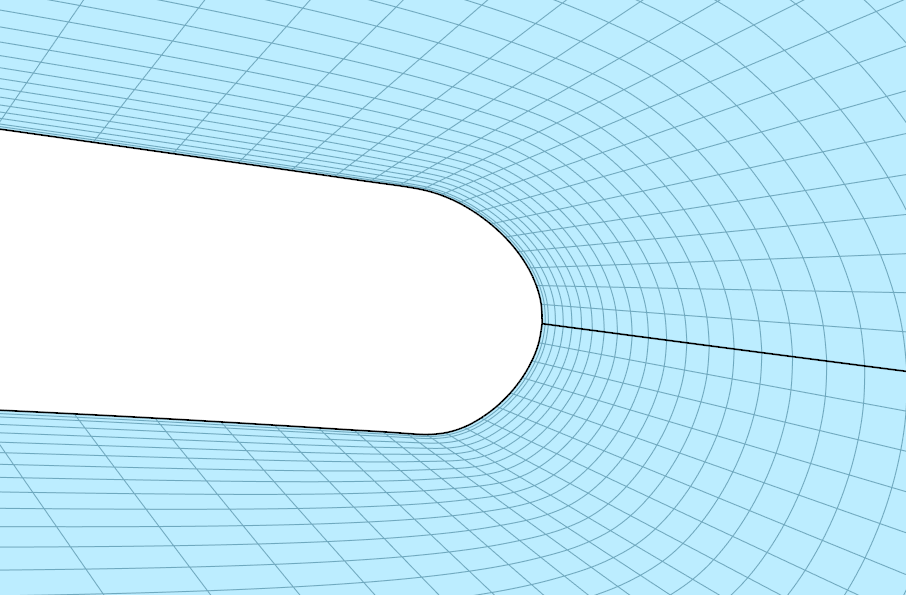
\includegraphics[width=0.6\textwidth]{figs/nonorthogonal}
  \end{figure}
\end{frame}

\begin{frame}
  \frametitle{Orthogonalized TFI}

  We ``grow'' the mesh layer by layer in the $v$-direction (radially out from the body). At each step:

  \begin{enumerate}
    \item Translate the points on the previous level some distance in the normal direction, giving
      $\mathbf{p}_{o,i}$.
    \item Compute the linear TFI as given by the previous curve $\mathbf{c}_1$, the outer curve
      $\mathbf{c}_2$ (which does not change), and sub-curves of $\mathbf{c}_3$ and $\mathbf{c}_4$.
      Evaluate it only for the next step in the $v$-direction, giving $\mathbf{p}_{t,i}$.
    \item Blend: $\mathbf{p}_i = (1-\alpha)\mathbf{p}_{o,i} + \alpha\mathbf{p}_{t,i}$.
  \end{enumerate}
\end{frame}

\begin{frame}
  \frametitle{Orthogonalized TFI}

  \only<1>{
    The blending factor $\alpha$ should be $1$ for the first $k$ steps (corresponding to the boundary
    layer), then decrease to zero, e.g.
    \[
    \alpha_j = \begin{cases} 1, & j \leq k, \\ 0, & j = N, \\ r_\alpha^{j-k}, & \text{otherwise.} \end{cases}
    \]
  }

  \only<2>{
    \begin{figure}
      \centering
      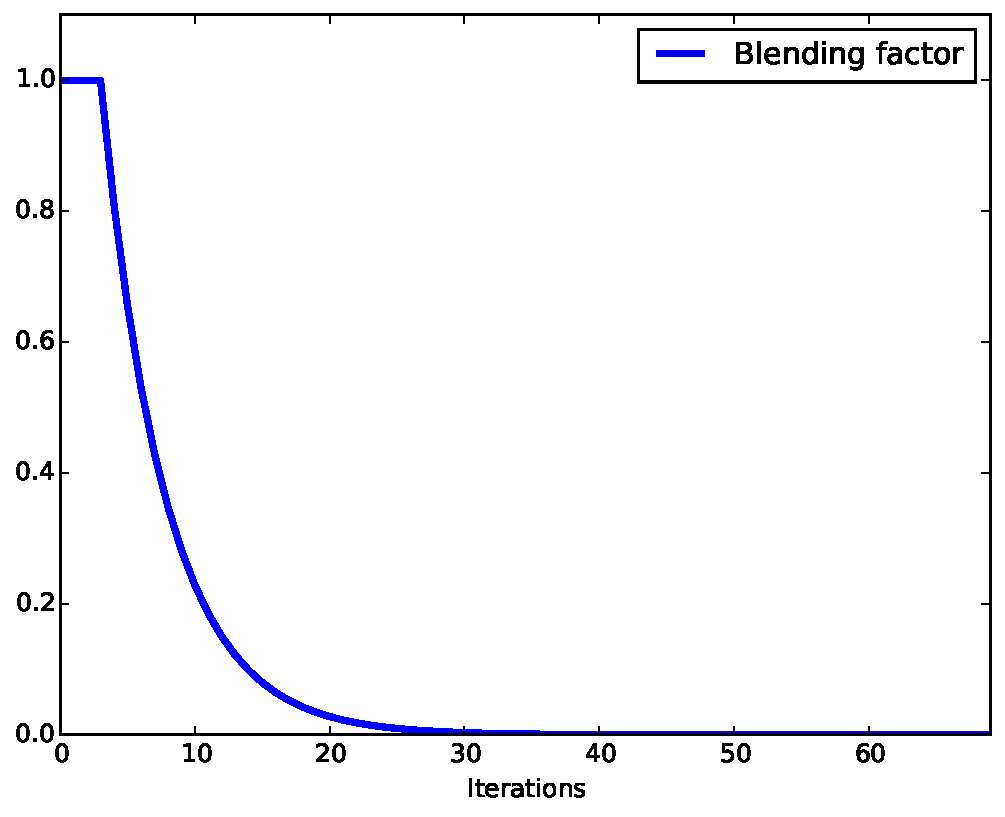
\includegraphics[width=0.5\textwidth]{figs/blending}
      \caption{$r_\alpha=0.81$, $k=4$, $N=70$.}
    \end{figure}
  }
\end{frame}

\begin{frame}
  \frametitle{Orthogonalized TFI}

  \begin{figure}
    \centering
    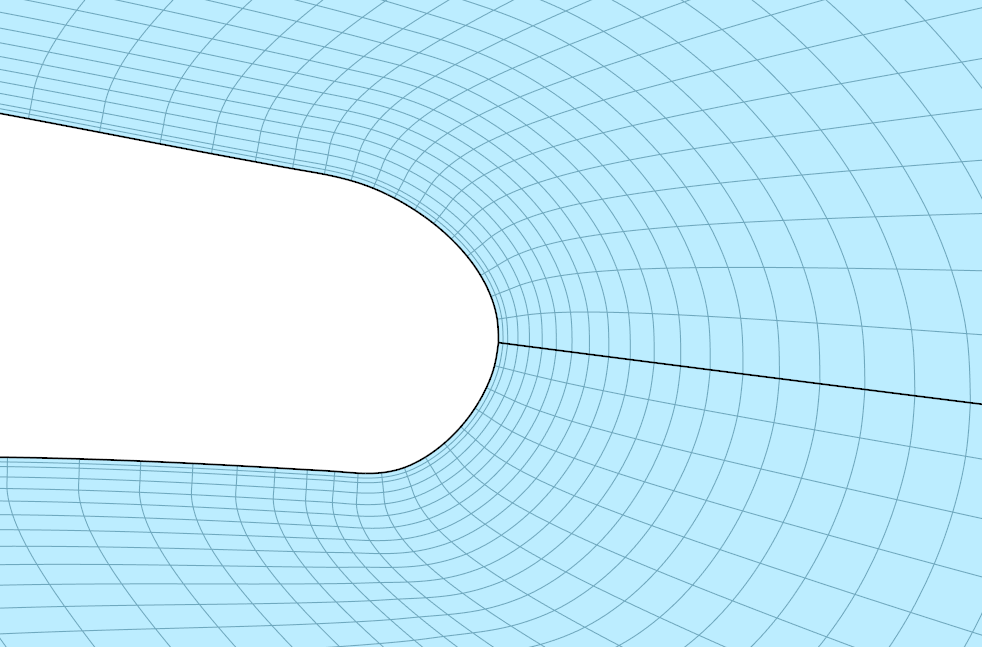
\includegraphics[width=0.7\textwidth]{figs/orthogonal}
  \end{figure}
\end{frame}

\subsection{Smoothing}

\begin{frame}
  \frametitle{Smoothed orthogonalized TFI}

  Problem: In rare cases, concavity can lead to crossing meshlines.

  \begin{figure}
    \centering
    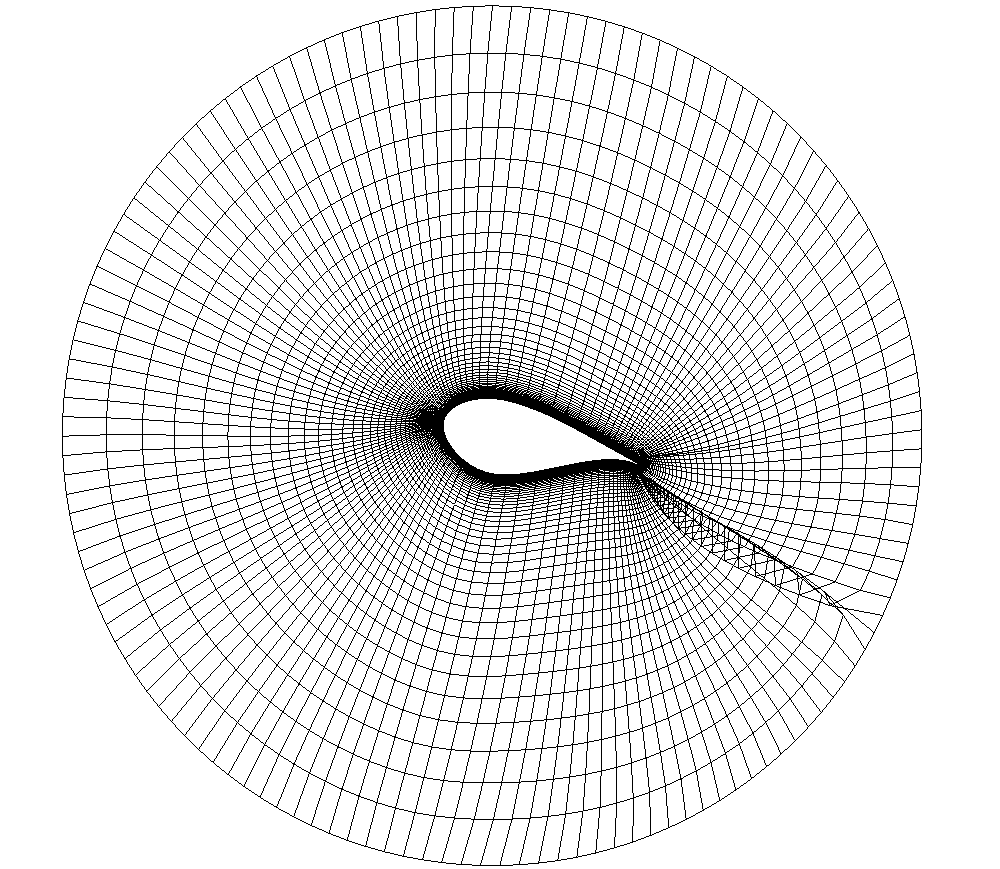
\includegraphics[width=0.5\textwidth]{figs/section12}
  \end{figure}
\end{frame}

\begin{frame}
  \frametitle{Smoothed orthogonalized TFI}

  \only<1>{
    At each step, perform a Laplacian smoothing on the points $\mathbf{p}_{o,i}$:
    
    \[
    \mathbf{p}_{s,i} = \mathbf{p}_{o,i} + \frac{1-\beta}{2} \left( 
      \mathbf{p}_{o,i+1} + \mathbf{p}_{o,i+1} - 2\mathbf{p}_{o,i}
    \right)
    \]

    Note: The smoothing has to happen ``on the curve''! \\~\\

    The smoothing factor $\beta$ should behave in a similar fashion as $\alpha$.
  }

  \only<2>{
    \begin{figure}
      \centering
      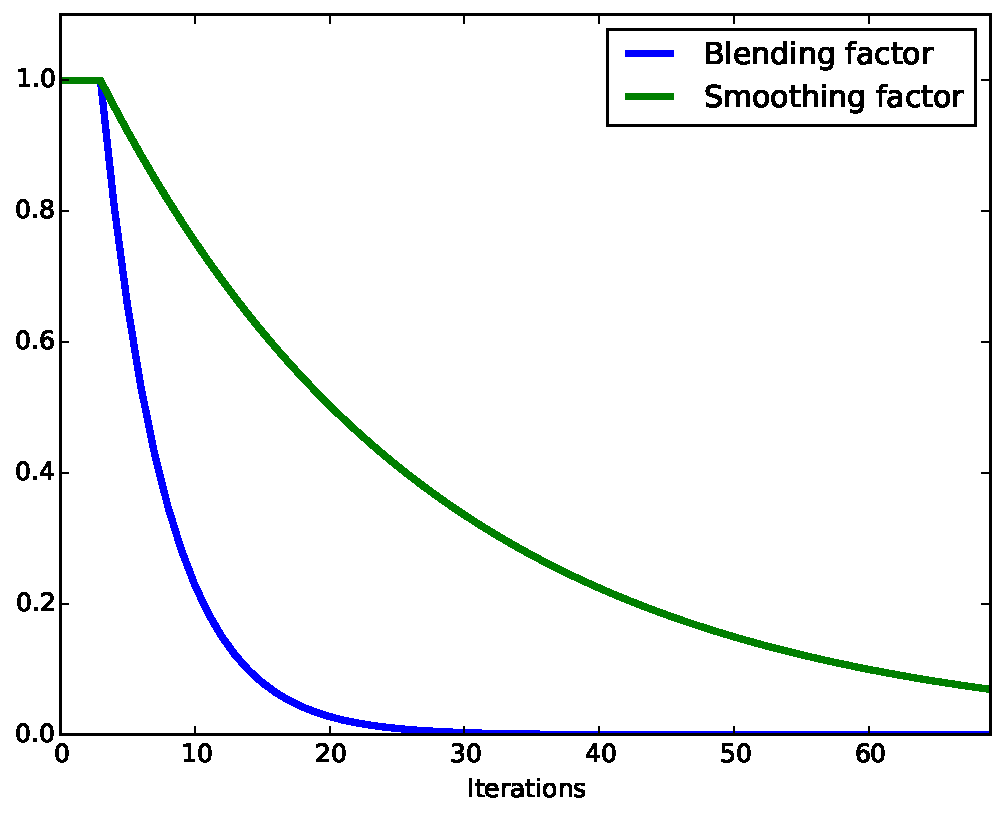
\includegraphics[width=0.5\textwidth]{figs/blending-smoothing}
      \caption{$r_\beta=0.96$, $k=4$, $N=70$.}
    \end{figure}
  }
\end{frame}

\begin{frame}
  \frametitle{Smoothed orthogonalized TFI}

  \begin{figure}
    \centering
    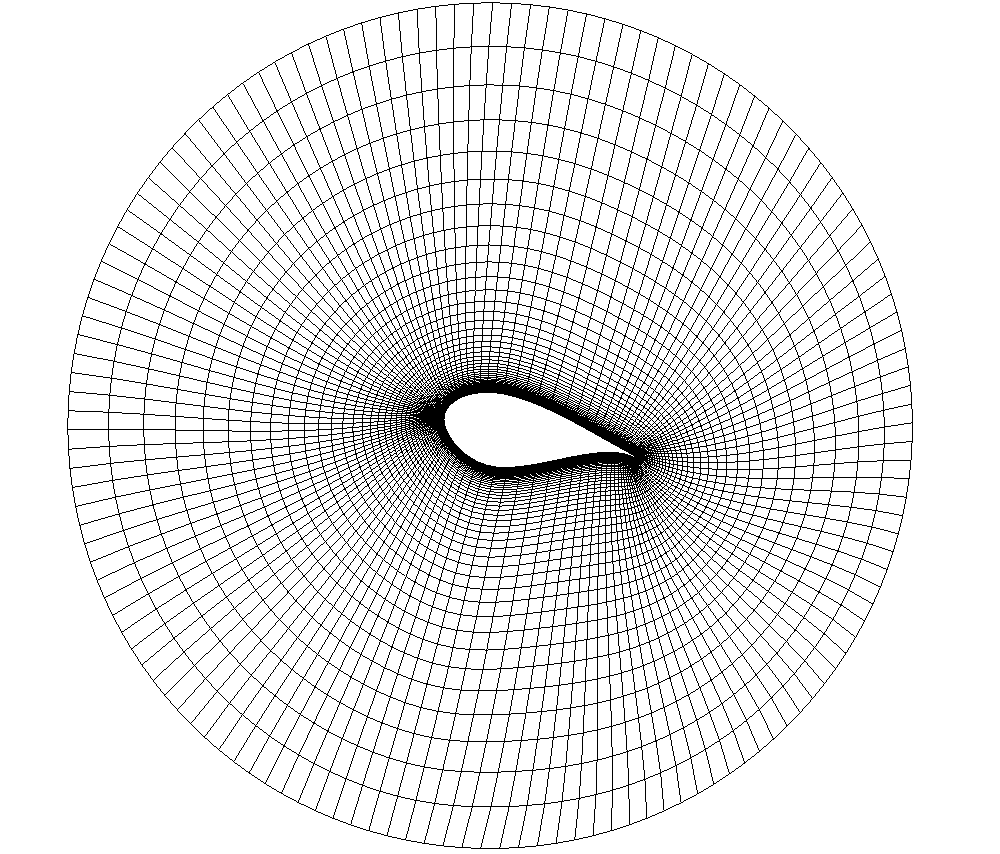
\includegraphics[width=0.5\textwidth]{figs/section12_smooth}
  \end{figure}
\end{frame}

\section{Wingtip}

\begin{frame}
  \frametitle{Wingtip}

  This produces an ``O''-mesh for every cross section, which can be lofted together.  The tip remains.

  \begin{figure}
    \centering
    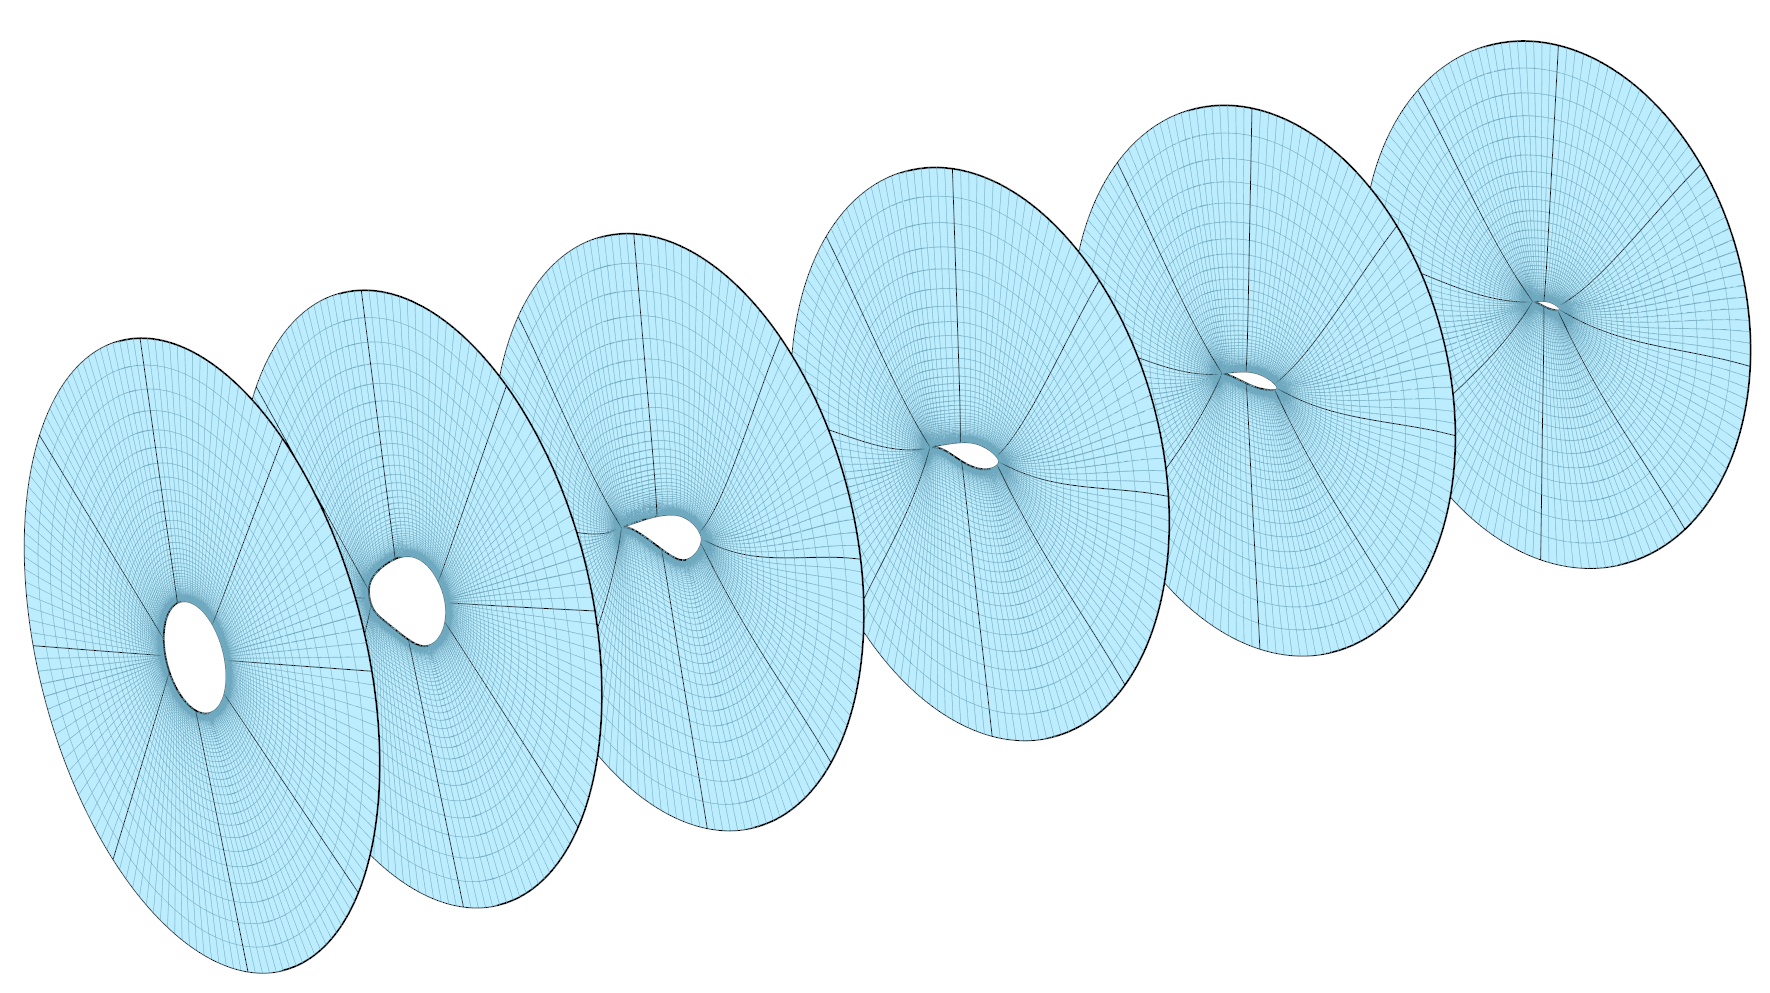
\includegraphics[width=0.7\textwidth]{figs/crossecs2}
  \end{figure}
\end{frame}

\begin{frame}
  \frametitle{Wingtip}

  \begin{figure}
    \centering
    \only<1>{
      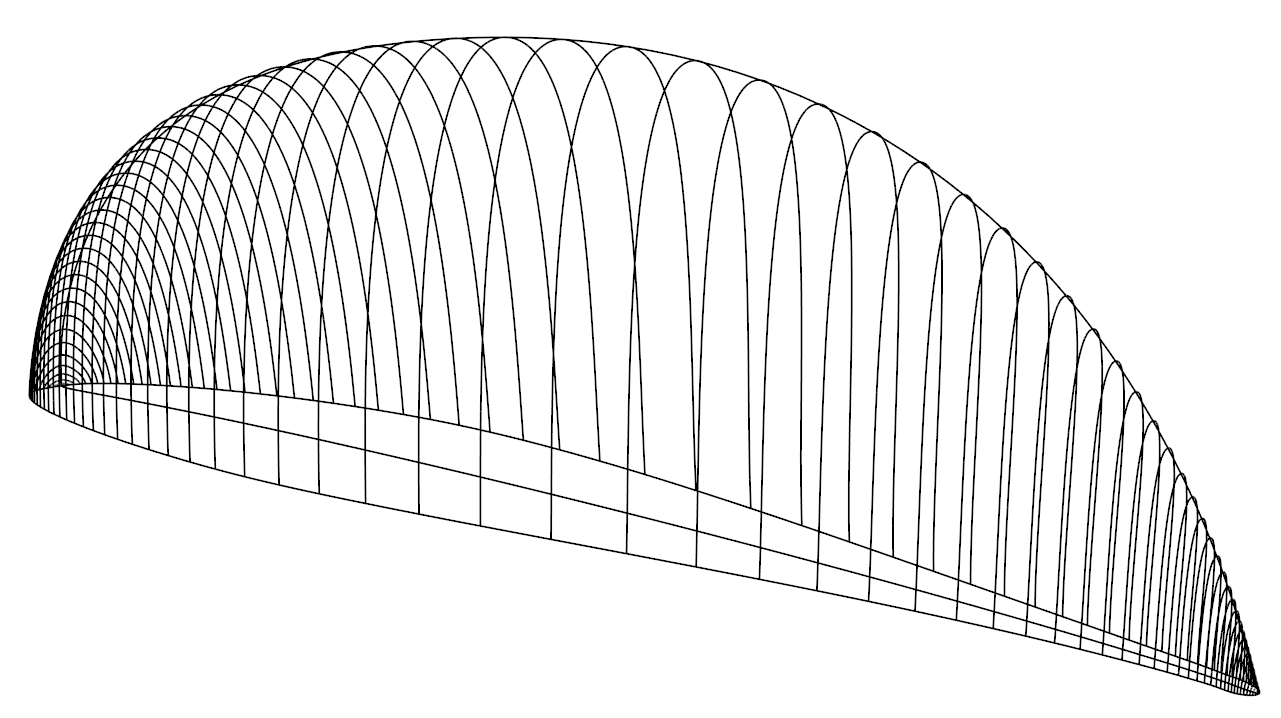
\includegraphics[width=0.7\textwidth]{figs/wingtip-skeleton}
      \caption{Lift the midline and form cross sections.  This gives a parametrized wingtip with singularities.}
    }
    \only<2>{
      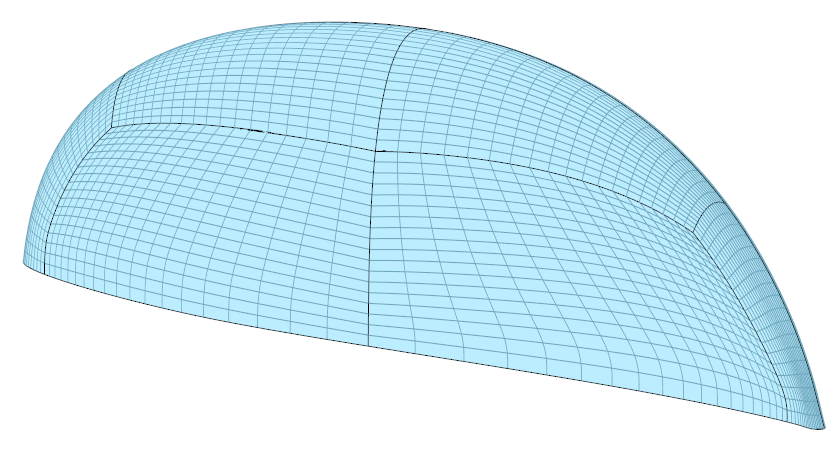
\includegraphics[width=0.7\textwidth]{figs/wingtip-full}
      \caption{Carefully section the tip into twelve patches, with no singularities.}
    }
  \end{figure}
\end{frame}

\begin{frame}
  \frametitle{Wingtip ``flower''}

  \begin{figure}
    \centering
    \only<1>{
      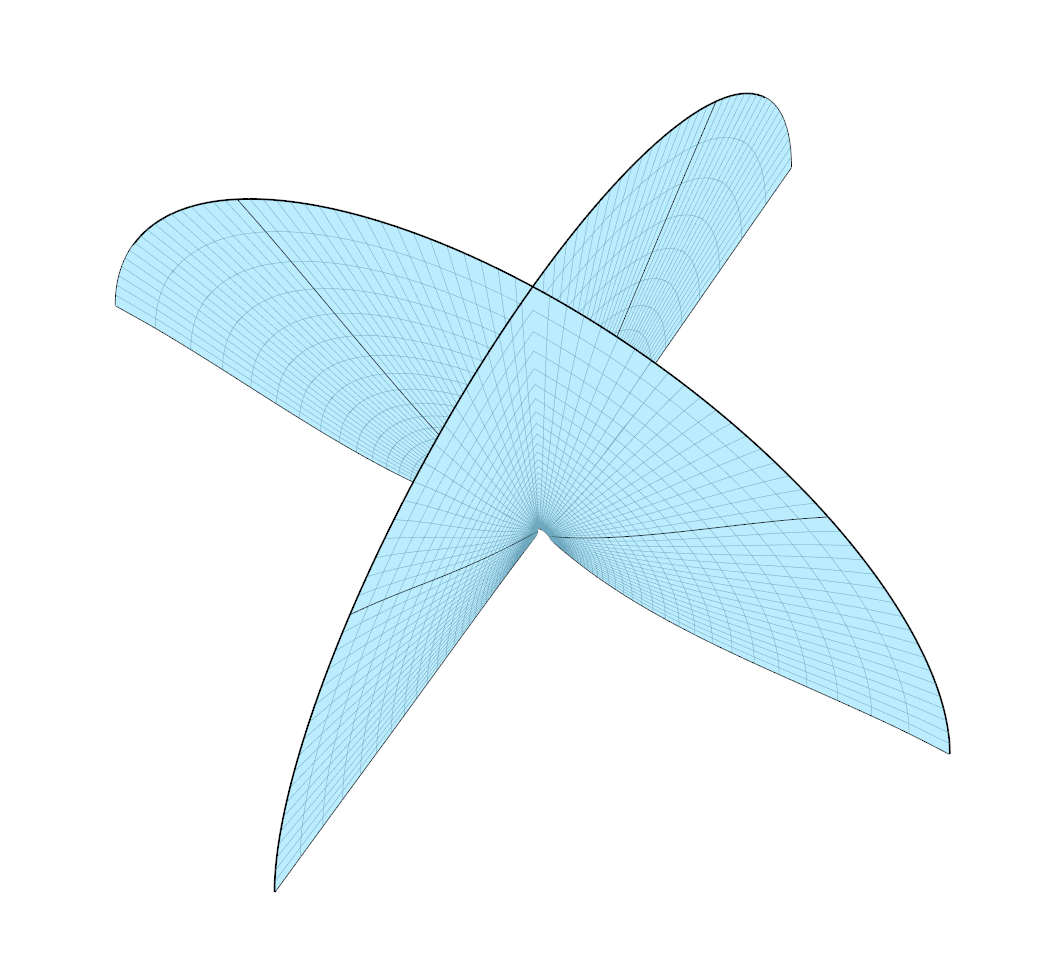
\includegraphics[width=0.5\textwidth]{figs/wingtip-first}
      \caption{Form the axial surfaces using TFI as described.}
    }
    \only<2>{
      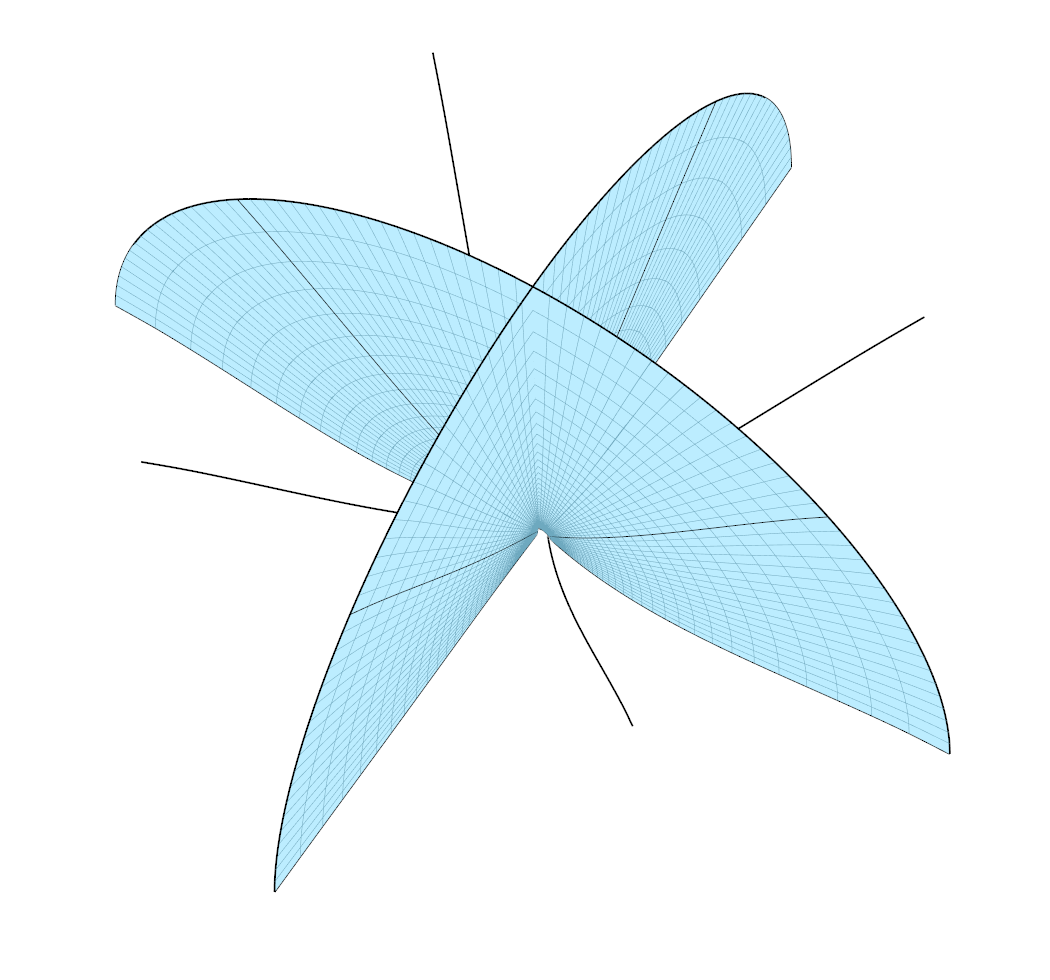
\includegraphics[width=0.5\textwidth]{figs/wingtip-centers}
      \caption{In each quadrant, create a suitable center curve.}
    }
    \only<3>{
      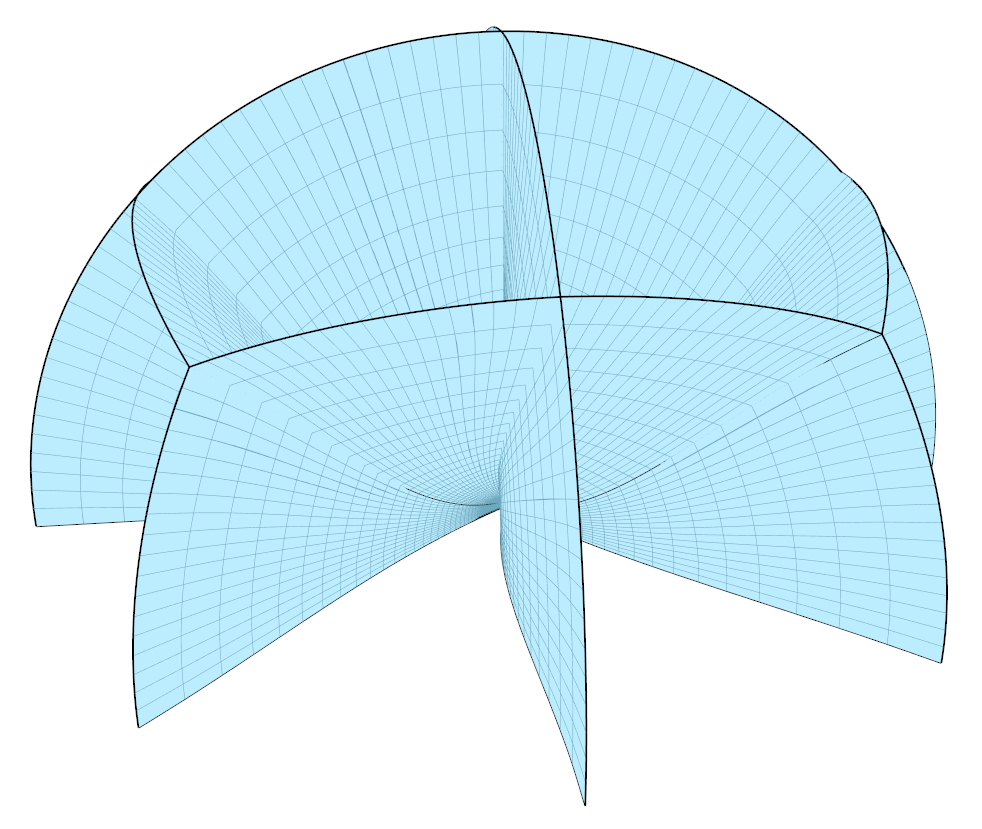
\includegraphics[width=0.5\textwidth]{figs/wingtip-flower}
      \caption{Complete the ``flower'' using TFI.  Use volumetric orthogonalized TFI to fill in the
        hemisphere.}
    }
  \end{figure}
\end{frame}

\section{Full mesh structure}

\begin{frame}
  \frametitle{Block structure}

  \begin{figure}
    \centering
    \only<1>{
      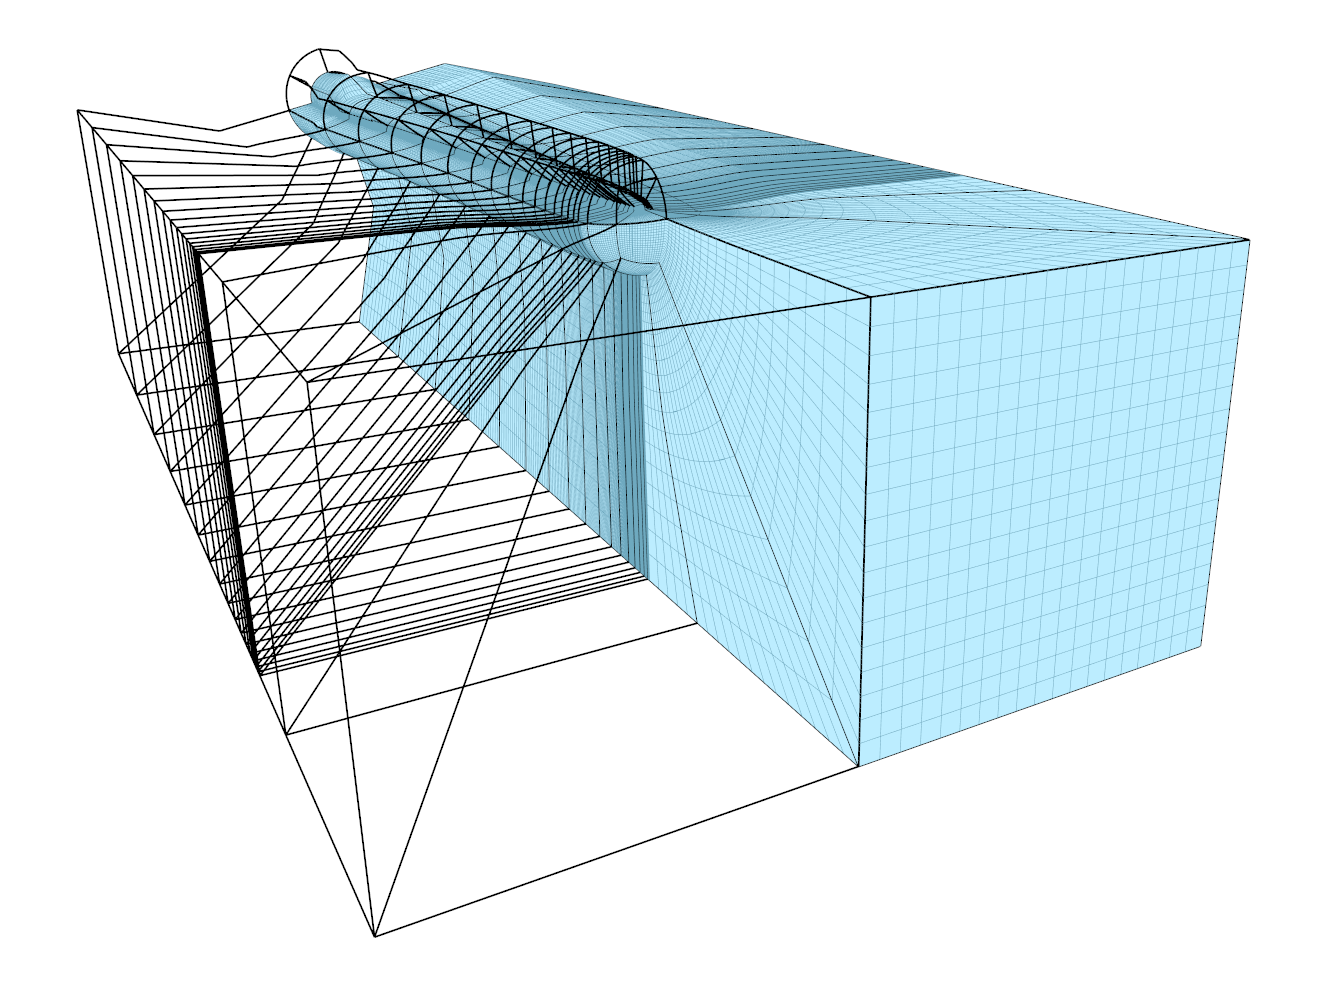
\includegraphics[width=0.7\textwidth]{figs/block-1}
    }
    \only<2>{
      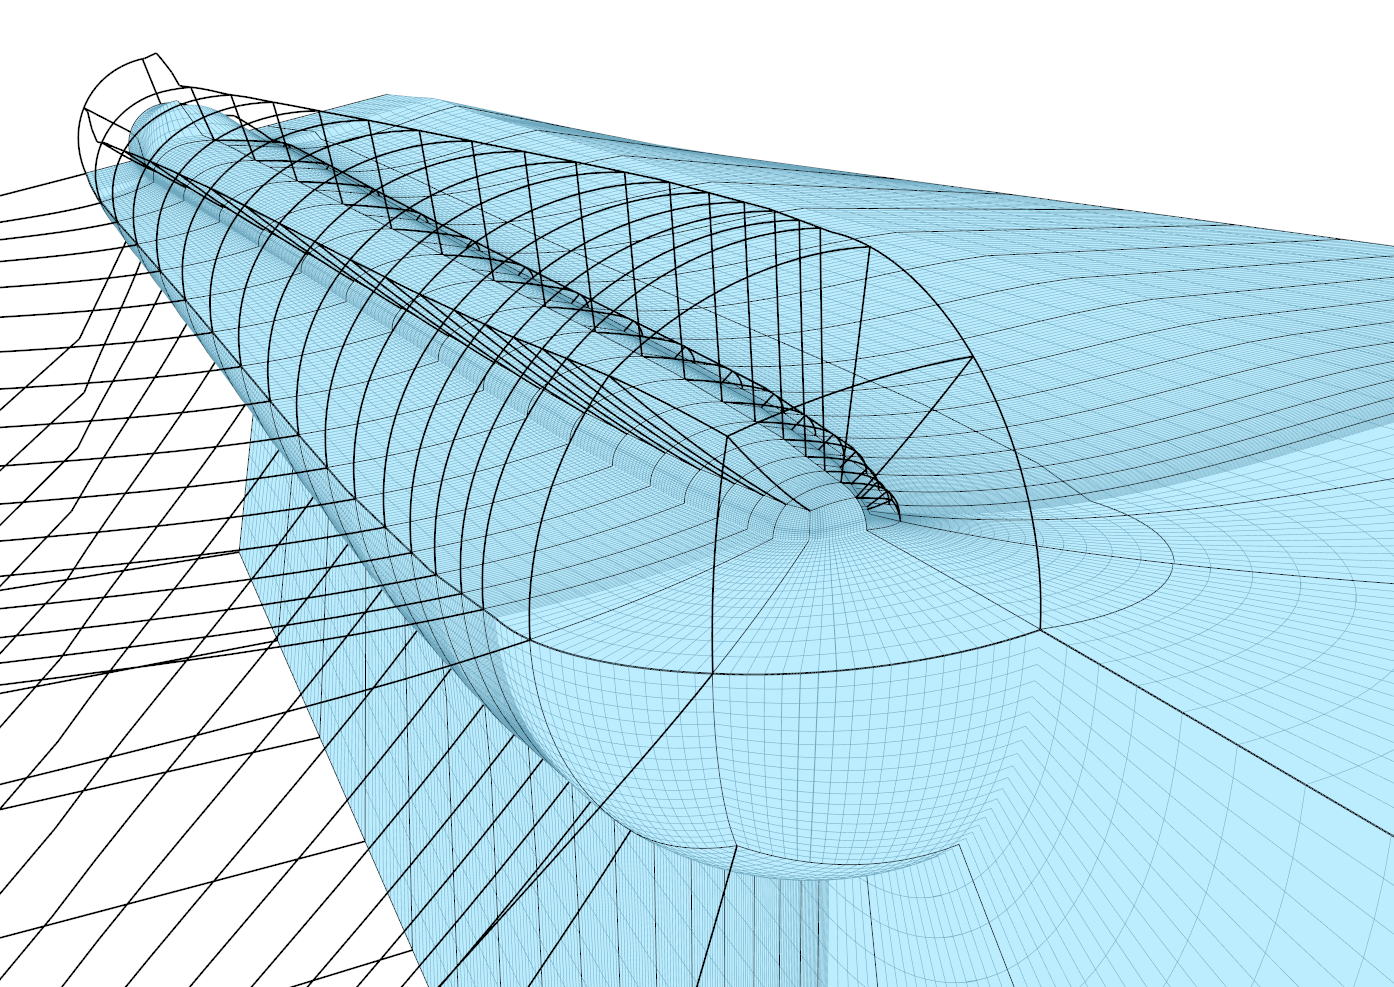
\includegraphics[width=0.7\textwidth]{figs/block-2}
    }
    \only<3>{
      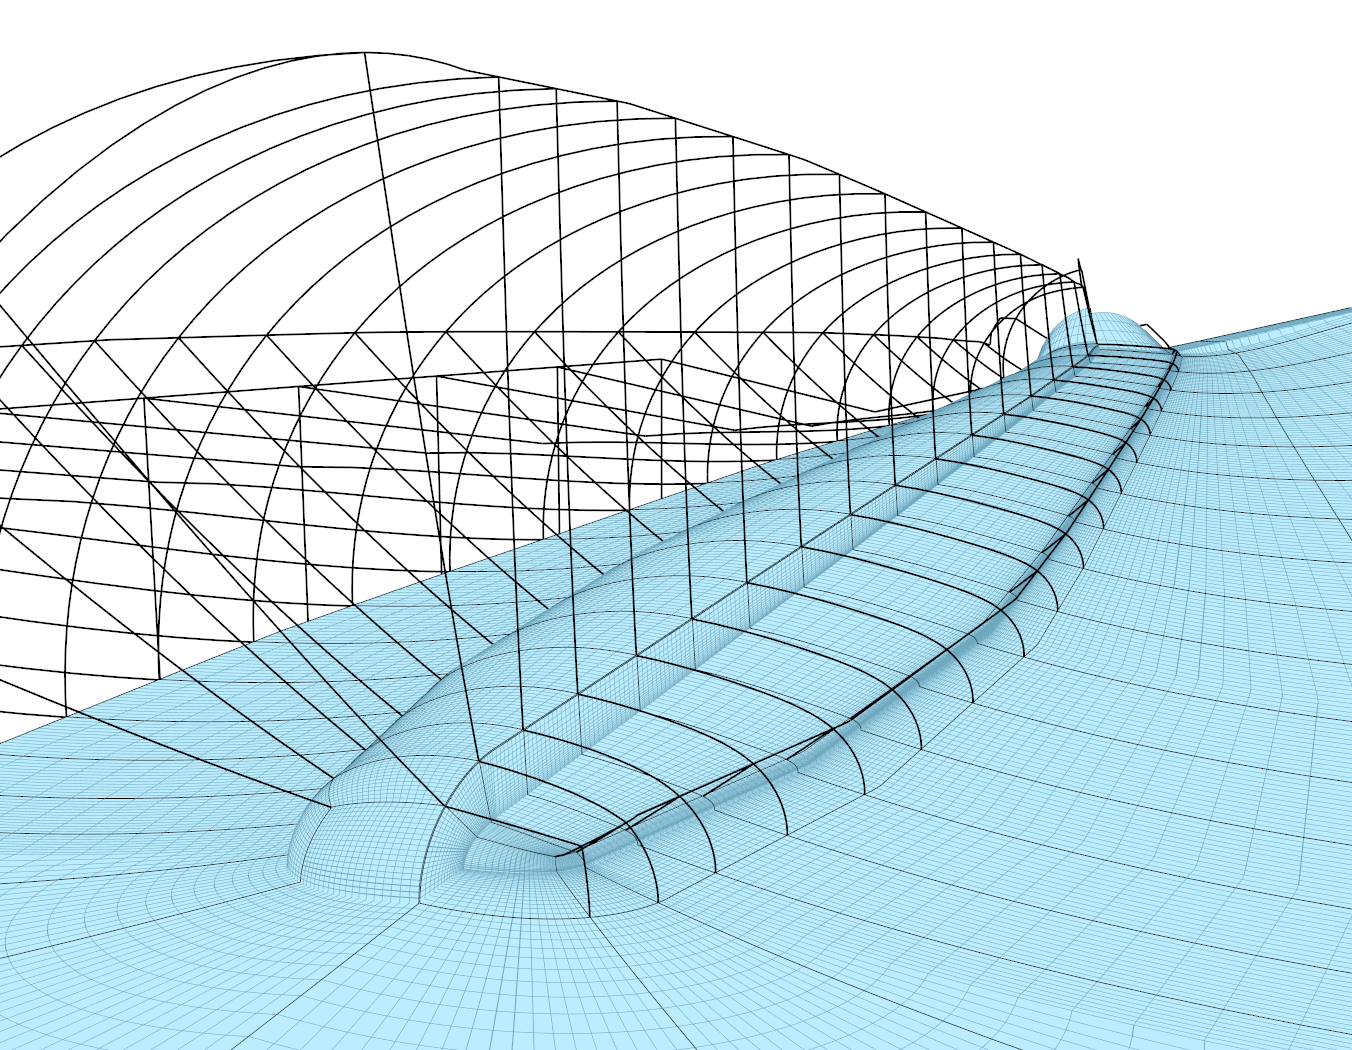
\includegraphics[width=0.7\textwidth]{figs/block-3}
    }
  \end{figure}
\end{frame}

\end{document}
